\subsection{Lautstärkeverarbeitung}\label{subsec:Volume_Generation}
Die Aufgabe der \textit{Lautstärkenverarbeitung} ist es aus dem Signal des Lautstärkenoszillators einen Dämpfungsfaktor zu berechnen, mit welchem das Signal der Tonhöhenverarbeitung multipliziert wird. So kann der Spieler die Lautstärke während dem Spielen wie die Tonhöhe über eine Antenne einstellen. Wie Abbildung \ref{img:Blockschaltbild_volume} zeigt sind die beiden Verarbeitungskomponenten auch sehr ähnlich. Der Referenzoszillator und der Mischer sind gleich wie in der Tonverarbeitung. In den nächsten Abschnitten sind die Unterschiede zu den Komponenten der Tonverarbeitung aufgezeigt.



\begin{figure}[h!]
	\centering
	\includegraphics[width=1\textwidth]{Blockschaltbild_Volume.pdf}
	\caption{Blockschaltbild der Custom IP Volume Generation} 
	\label{img:Blockschaltbild_volume}
\end{figure}  

\paragraph{Filter}\mbox{}\\
Beim \textit{Filter} der Laustsärkeverarbeitung wurde die Frequenzmessung erst nach dem dritten CIC Filter angeschlossen. Wir haben dies so gemacht, um beim FIR-Filter der Frequenzmessungskomponente weniger Koeffizienten und somit weniger Ressourcen zu benötigen. Das FIR-Filter benötigt deshalb weniger Koeffizienten, da nach CIC 3 die Abtastfrequenz des Signals um den Faktor 45 kleiner ist. Zudem ist das FIR-Filter in dieser Komponente deshalb nicht mehr nötig.

\begin{figure}[h!]
	\centering
	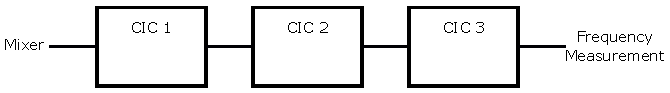
\includegraphics[width=0.8\textwidth]{Filter_volume.pdf}
	\caption{Aufbau des Filters in der Komponente Volume Generation} 
	\label{img:Filter_Volume}
\end{figure}  

\paragraph{Frequenzmessung \& Kalibration}\mbox{}\\
Auch bei der Komponente \textit{Frequenzmessung} waren Anpassungen nötig.

\begin{figure}[h!]
	\centering
	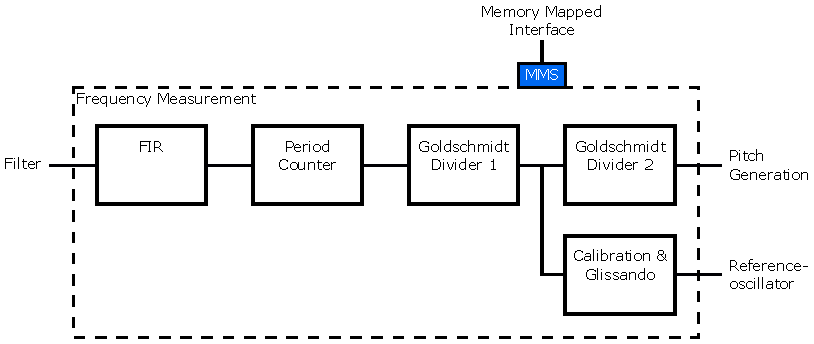
\includegraphics[width=1\textwidth]{freq_meas_volume.pdf}
	\caption{Aufbau der Frequenzmessung und Kalibration in der Komponente Volume Generation} 
	\label{img:freq_meas_volume}
\end{figure}  